\chapauthor{Никифоров С.А.\\Гойло А.А.\\Крощенко А.А.\\Захарьев В.А.\\Цянь Л.}
\chapter{Естественно-языковые интерфейсы ostis-систем}
\chapauthortoc{Никифоров С.А.\\Гойло А.А.\\Крощенко А.А.\\Захарьев В.А.\\Цянь Л.}
\label{chapter_nl_interfaces}

\abstract{
    В данной главе рассматривается подход к реализации естественно-языковых интерфейсов интеллектуальных компьютерных систем нового поколения, построенных по технологии OSTIS, а также предлагается модель контекста диалога.
    В данном подходе все этапы анализа, включая лексический, синтаксический и семантический анализ могут производиться непосредственно в базе знаний такой системы. Такой подход позволит эффективно решать такие задачи как управление глобальным и локальным контекстами диалога, а также разрешение языковых явлений таких как анафоры, омонимия и эллиптические фразы.

    \begin{textitemize}
        \item расписать сопоставление токенов с лексемами;
        \item перерисоват ькартинки, чать из них предназначалась для размещения в колонке;
        \item расписать синтаксический анализ, как находятся составляющие,
        \item пройтись по подсказкам от плагина, поправит форматирование,
        \item формализовать пр. о..
    \end{textitemize}
    Список вопросов:
    \begin{textitemize}
        \item что придумать с аналогичными картинками, как те, что были использованы в главе про языки - дублировать в одной книге плохо, но ссылаться чрез 100 страниц тоже.
    \end{textitemize}
}

%Введение
В настоящее время существует большое количество различных интерфейсов компьютерных систем, что усложняет интероперабельность между такими системами и людьми в силу необходимости ознакомления с интерфейсом каждой новой системы, который зачастую может быть не интуитивно понятен.

Одной из основных особенностей интеллектуальных компьютерных систем нового поколения должен являться пользовательский интерфейс, способный обеспечить эффективное взаимодействие пользователя с системой в условиях его общей профессиональной неподготовленности.

Одной из наиболее естественных и удобных форм передачи информации между людьми является речь, что обуславливает все большее распространение естественно-языковых интерфейсов\scncite{GlobalMarket}. В настоящий момент времени уже ни у кого не вызывает сомнения, что данная форма взаимодействия человека и машины играет и будет играть значительную роль во взаимодействии с различными компьютерными системами.

Однако необходимо отметить, что большое многообразие языков (как естественных, так и искусственных) ведет к необходимости упрощения процесса создания таких интерфейсов для каждого отдельно взятого языка.

%Анализ
В основе большинства подходов к обработке и пониманию естественного языка лежит машинное обучение\scncite{NLP_as_a_service},\scncite{NLP_in_pharmacology}. Несомненно, для большинства широко распространенных языков модели для обработки естественного языка работают очень хорошо и совершенствуются с каждым днем, но несмотря на успехи в данной области, данный подход имеет ряд недостатков:
\begin{textitemize}
    \item проблемы при работе с различными областями, например, значения слов или предложений могут быть различными в зависимости от предметной области. Таким образом, модели для NLP могут хорошо работать для отдельной предметной области, но не подходить для широкого применения\scncite{NLPOverview};
    \item создание новой модели модели требует наличия большого объема данных, а качество таких данных напрямую влияет на качество получаемой модели, что ведет к большим затратам на ее обучение\scncite{strubell2019energy}\scncite{large_language_models};
    \item данные модели представляют собой "черный ящик"{}, т. к. данные модели не обладают средствами для обоснования своего вывода;
    \item каждая такая модель решает только свой узкий класс задач, отсутствует общий подход к обработке естественного языка.\scncite{NLPOverview}
\end{textitemize}

Данные недостатки используемых методов являются причиной части недостатков современных систем, реализующих естественно-языковой интерфейс, так, несмотря на то, что сейчас существует большое количество речевых ассистентов, создаваемых разными компаниями\scncite{site_url_alexa},\scncite{site_url_siri},\scncite{site_url_gassist},\scncite{site_url_cortana}, они обладают схожими недостатками, например, исключительно распределенной реализацией, в силу недостаточной для запуска ресурсоемких моделей производительности устройств конечных пользователей. Это в свою очередь ведет к проблемам с приватностью\scncite{PVA}.

Подмодуль понимания речи данных систем формирует конструкцию, отражающую смысл сообщения используя фреймовую модель. Упрощенный пример такой конструкции приведен на рисунке \textit{\nameref{fig:message_intents}}.

\begin{figure}[h]
    \centerline{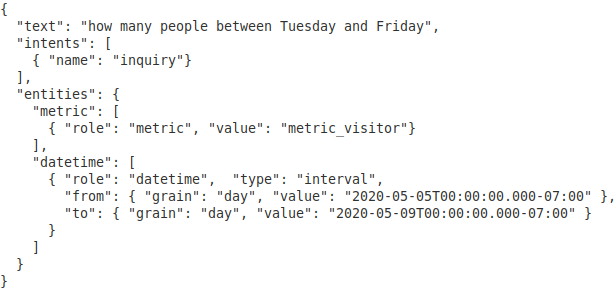
\includegraphics[width=\linewidth]{images/part4/chapter_nl_interfaces/message_intents.png}}
    \caption{Пример формализованного смысла сообщения}
    \label{fig:message_intents}
\end{figure}

При этом для представления результатов промежуточных этапов обработки используются иные форматы, модули которые их реализуют не имеют какой-либо единой основы и взаимодействуют посредством специализированных программных интерфейсов между ними, что приводит к несовместимости способов представления результатов на различных этапах обработки и конечного результата обработки текстов. Данная несовместимость в свою очередь ведет к существенным накладным расходам при разработке такой системы и в особенности при ее модификации.

В качестве решения проблемы совместимости предлагается использование подхода к обработке естественного языка на основе его формальной модели в виде набора онтологий, сформированных с использованием универсальных средств представления знаний, что будет способствовать интероперабельности как компонента по обработке естественного языка в целом с другими компонентами системы, так и между составляющими самого данного компонента.

Целью главы является формирование модели интерфейса, в основе которой лежит подход к обработке естественного языка на основе онтологий, содержащих формальное описание естественного языка.

\section{Предметная область и онтология естественно-языковых интерфейсов ostis-систем}

\textit{Естественно-языковой интерфейс} -- SILK-интерфейс (Speech – речь, Image – образ, Language – язык, Knowledge – знание), обмен информацией между компьютерной системой и пользователем в котором происходит за счёт диалога. Диалог ведётся на одном из естественных языков.

\begin{SCn}

    \scnheader{естественно-языковой интерфейс}
    \scnsuperset{речевой интерфейс}

\end{SCn}

\textit{Речевой интерфейс} -- SILK-интерфейс, обмен информацией в котором происходит за счёт диалога, в процессе которого компьютерная система и пользователь общаются с помощью речи. Данный вид интерфейса наиболее приближен к естественному общению между людьми.

В предлагаемом подходе можно выделить следующие этапы обработки естественного языка:
\begin{textitemize}
    \item лексический анализ;
    \item синтаксический анализ;
    \item понимание сообщения.
\end{textitemize}

В свою очередь, лексический анализ в включает в себя декомпозицию текста на токены и их сопоставление с лексемами.

Понимание сообщения сводится к генерации вариантов значения сообщения и выбору из них корректного на основании контекста, а также погружение его в данный контекст.

Ниже приведена структура решателя задач естественно-языкового интерфейса.

\begin{SCn}

    \scnheader{Решатель задач естественно-языкового интерфейса}
    \begin{scnrelfromset}{декомпозиция абстрактного sc-агента}
        \scnitem{Абстрактный sc-агент лексического анализа}
        \begin{scnindent}
            \begin{scnrelfromset}{декомпозиция абстрактного sc-агента}
                \scnitem{Абстрактный sc-агент декомпозиции текста на токены}
                \scnitem{Абстрактный sc-агент сопоставления токенов с лексемами}
            \end{scnrelfromset}
        \end{scnindent}
        \scnitem{Абстрактный sc-агент синтаксического анализа}
        \scnitem{Абстрактный sc-агент понимания сообщения}
    \end{scnrelfromset}

\end{SCn}

В свою очередь, \textit{Абстрактный sc-агент понимания сообщения} декомпозируется на:

\begin{SCn}

    \scnheader{Агент понимания сообщения}
    \begin{scnrelfromset}{декомпозиция абстрактного sc-агента}
        \scnitem{Абстрактный sc-агент генерации вариантов значения сообщения}
        \scnitem{Абстрактный sc-агент выбора и обновления контекста}
        \begin{scnindent}
            \begin{scnrelfromset}{декомпозиция абстрактного sc-агента}
                \scnitem{Абстрактный sc-агент разрешения контекста}
                \scnitem{Абстрактный sc-агент выбора смысла сообщения на основе контекста}
                \scnitem{Абстрактный sc-агент погружения сообщения в контекст}
            \end{scnrelfromset}
        \end{scnindent}
    \end{scnrelfromset}

\end{SCn}

Для каждого агента в базе знаний должна находиться спецификация, пример фрагмента такой спецификации приведен на рисунке \textit{\nameref{fig:agent_spec}}.

\begin{figure}[h]
    \centering
    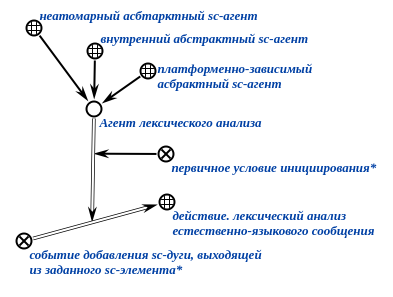
\includegraphics[width=0.4\textwidth]{images/part4/chapter_nl_interfaces/agent_spec.png}
    \caption{Пример спецификации агента.}
    \label{fig:agent_spec}
\end{figure}

\section{Предметная область и онтология лексического анализа естественно-языковых сообщений, входящих в ostis-систему}

\begin{SCn}

    \scnheader{действие. лексический анализ естественно-языкового сообщения}
    \begin{scnrelfromset}{обобщенная декомпозиция}
        \scnitem{действие. декомпозиция текста на токены}
        \scnitem{действие. сопоставление токенов с лексемами}
    \end{scnrelfromset}

\end{SCn}

С точки зрения ostis-системы, любой естественно-языковой текст является \textit{файлом} (т.е. SC-узлом с содержимым).

Этап лексического анализа представляет собой декомпозицию текста на последовательность токенов и сопоставление лексем с получившимися при данной декомпозиции токенами. Следует отметить, что данные токены при необходимости могут сопоставляться не с лексемами, а с их подмножествами, входящими в ее морфологическую парадигму, соответствующими определенным грамматическим категориям: падежу, числу, роду и т.д.

Результат лексического анализа представлен на рисунке \textit{\nameref{fig:lexical_result}}.

\begin{figure}[h]
    \centering
    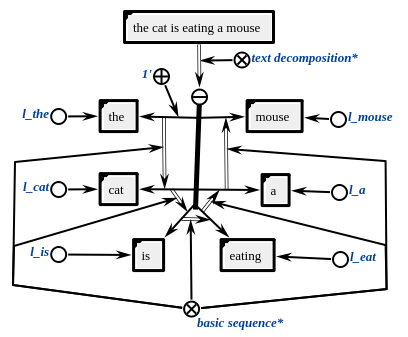
\includegraphics[width=0.4\textwidth]{images/part4/chapter_nl_interfaces/lexical.png}
    \caption{Пример результата лексического анализа.}
    \label{fig:lexical_result}
\end{figure}

Для осуществления лексического анализа, в базе знаний системы также должен присутствовать словарь, содержащий лексемы и их различные формы.

Под лексемой понимается единица словарного состава языка, которая представляет собой множество всех форм некоторого слова.
Пример спецификации лексемы в базе знаний приведен на рисунке \textit{\nameref{fig:lexeme_example}}.

\begin{figure}[h]
    \centering
    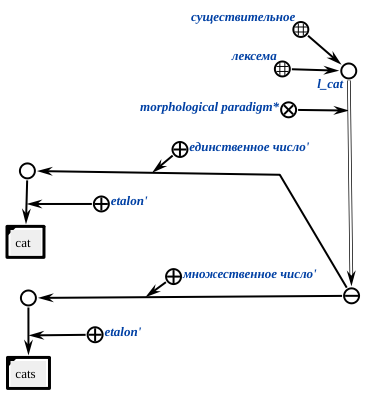
\includegraphics[width=0.4\textwidth]{images/part4/chapter_nl_interfaces/lexeme_example.png}
    \caption{Пример спецификации лексемы в базе знаний.}
    \label{fig:lexeme_example}
\end{figure}

\section{Предметная область и онтология синтаксического анализа естественно-языковых сообщений, входящих в ostis-систему}

Агент синтаксического анализа выполняет переход от размеченного на лексемы текста к его синтаксической структуре.
При этом из-за невозможности разрешения структурной неоднозначности на этапе синтаксического анализа, его результатом в общем случае будет являться множество потенциальных синтаксических структур.

Пример одной синтаксической структуры представлен на рисунке \textit{\nameref{fig:syntactic_result}}.

\begin{figure*}[h]
    \centering
    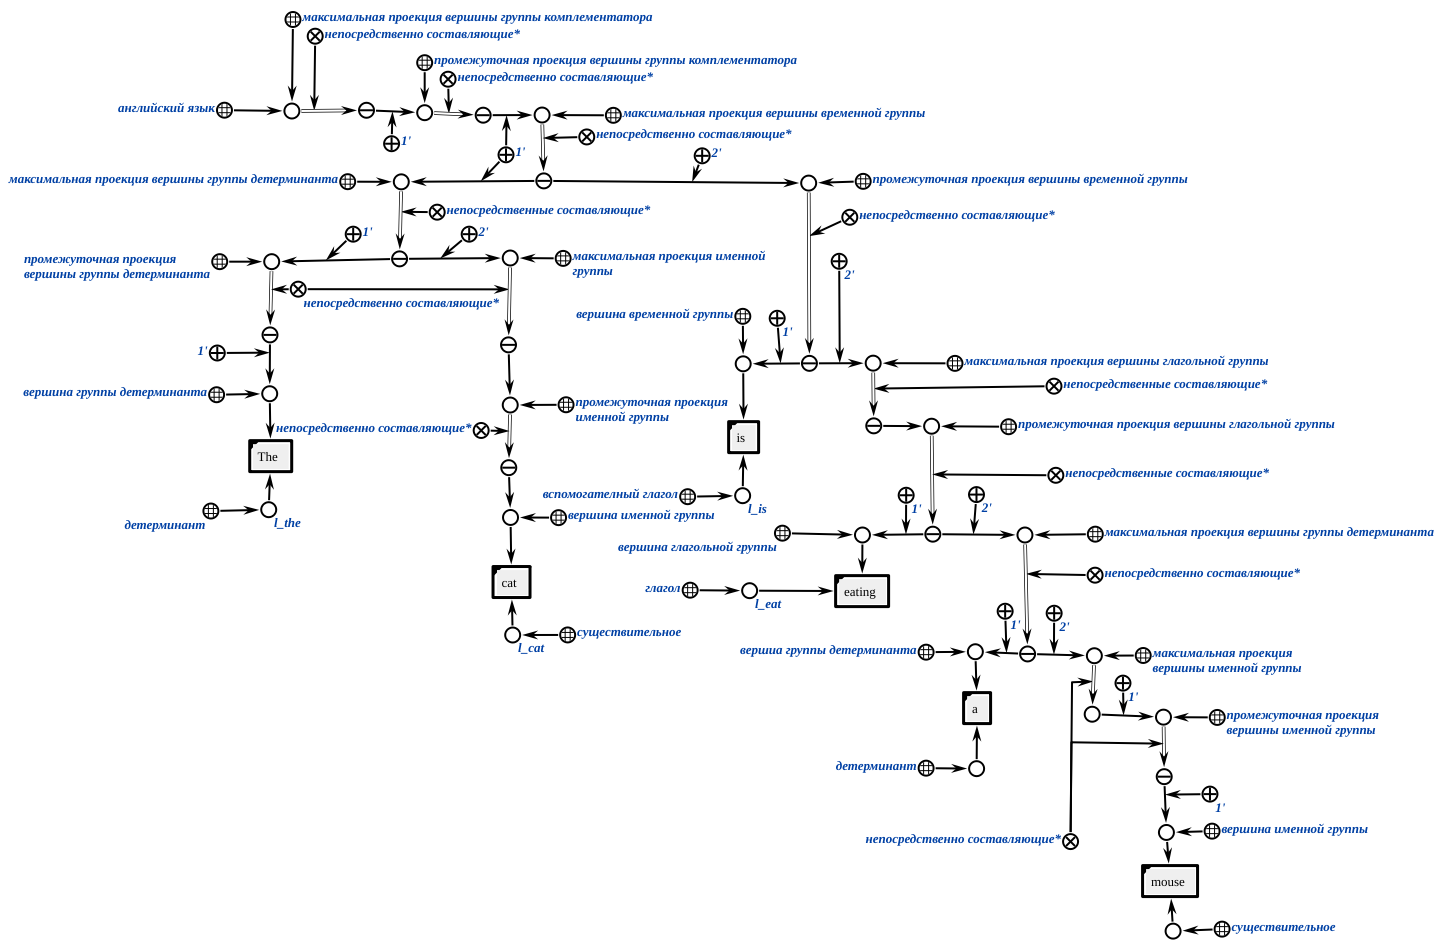
\includegraphics[width=\textwidth]{images/part4/chapter_nl_interfaces/syntactic.png}
    \caption{Пример синтаксической структуры.}
    \label{fig:syntactic_result}
\end{figure*}


\section{Предметная область и онтология понимания естественно-языковых сообщений, входящих в ostis-систему}

\begin{SCn}

    \scnheader{действие. понимание естественно-языкового сообщения}
    \begin{scnrelfromset}{обобщенная декомпозиция}
        \scnitem{действие. генерация вариантов значения сообщения}
        \scnitem{действие. выбор и обновление контекста}
        \begin{scnindent}
            \begin{scnrelfromset}{обобщенная декомпозиция}
                \scnitem{действие. разрешение контекста}
                \scnitem{действие. выбор смысла сообщения на основе контекста}
                \scnitem{действие. погружение сообщения в контекст}
            \end{scnrelfromset}
        \end{scnindent}
    \end{scnrelfromset}

\end{SCn}

\textit{Действие. генерация вариантов значения сообщения} -- действие, в ходе которого осуществляется формирование строгой дизъюнкции потенциально эквивалентных структур.

\textit{Потенциально эквивалентная структура*} -- бинарное ориентированное отношение, связывающее структуру и множество структур, которые потенциально могут быть эквивалентны ей, однако для достоверного определения факта требуются дополнительные действия.

При этом, переход от результата синтаксического анализа к потенциально эквивалентным сообщению структурам осуществляется по правилам, содержащихся в предметной области денотационной семантики. Пример одного из правил представлен на рисунке \textit{\nameref{fig:transition_to_semanic_rule}}.

\begin{figure*}[h]
    \centering
    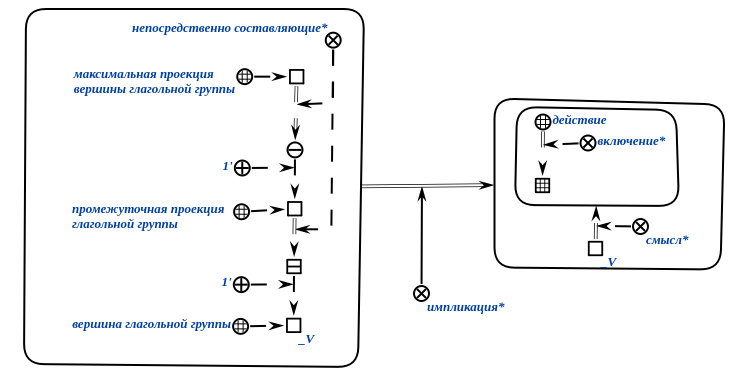
\includegraphics[width=0.7\textwidth]{images/part4/chapter_nl_interfaces/d_sem_3.png}
    \caption{Пример правила перехода от синтаксической структуры к семантике.}
    \label{fig:transition_to_semanic_rule}
\end{figure*}

В результате данного действия в базе знаний формируется структура, описывающая возможные варианты смысла сообщения, пример такой структуры в терминах грамматики составляющих\scncite{X_bar_syntax} приведен на \textit{\nameref{fig:messsage_meaning_variants}}. Наличие нескольких таких структур объясняется тем, что в общем случае на этапе синтаксического анализа выполняется генерация нескольких вариантов синтаксической структуры. Выбор корректного значения сообщения будет осуществлен в ходе выполнения последующих действий.

\begin{figure}[h]
    \centering
    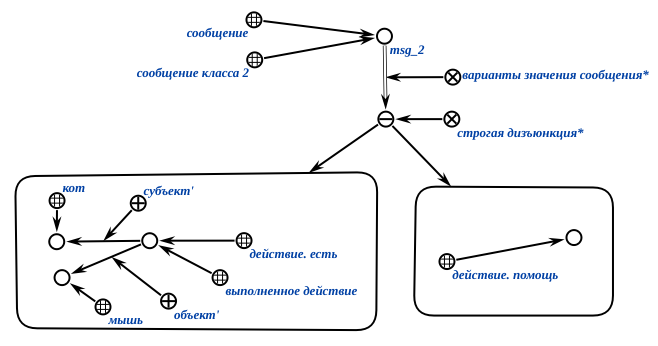
\includegraphics[width=0.45\textwidth]{images/part4/chapter_nl_interfaces/messsage_meaning_variants.png}
    \caption{Пример конструкции, описывающей потенциальные смыслы сообщения.}
    \label{fig:messsage_meaning_variants}
\end{figure}

Следует отметить, что при необходимости смысл сообщения может быть сгенерирован не только на основании его синтаксической структуры в терминах грамматики составляющих, но и других знаний о данном сообщении, например выделенных из текста данного сообщения троек вида субъект-отношение-объект, результата его классификации и т. п.

Дальнейшие этапы процесса понимания сообщения выполняются на основе контекста.

\textit{Контекст} - sc-структура, содержащая знания, которыми оперирует система в ходе одного или нескольких диалогов.
В общем случае, данные знания включают в себя как предварительно занесенные в БЗ, так и полученные в ходе работы с сенсоров и/или диалога.

\begin{SCn}

    \scnheader{контекст диалога}
    \scnsubset{контекст}
    \scnrelfrom{subdividing}{\scnkeyword{Типология контекстов диалога по глобальности\scnsupergroupsign}}
    \begin{scnindent}
        \begin{scneqtoset}
            \scnitem{тематический контекст}
            \scnitem{пользовательский контекст}
            \scnitem{глобальный контекст}
        \end{scneqtoset}
    \end{scnindent}

\end{SCn}

\textit{Тематический контекст} -- контекст диалога, содержащий специфические для темы сведения (сведения, полученные во время ведения диалога, на определенную тематику, например, при диалоге об определенном наборе сущностей).

\textit{Множество тематических контекстов диалога*} -- бинарное ориентированное отношение, диалог с ориентированным множеством его тематических контекстов.

\textit{Пользовательский контекст} -- контекст диалога, содержащие специфические для пользователя сведения, которые могут быть использованы в диалоге с ним на любую тематику. В общем случае пользовательский контекст имеет пересечение с согласованной частью БЗ (предварительно занесенная в БЗ достоверная информация о пользователе, прошедшая необходимую модерацию), но не включается в нее целиком (часть, полученная в ходе диалога в которой мы не уверены).
Пример соотнесения различных типов контекстов с согласованной частью базы знаний приведен на рисунке \textit{\nameref{fig:context_in_KB}}.

\textit{Глобальный контекст} -- контекст диалога, содержащий сведения, которые могут быть необходимы при ведении диалога с любым пользователем. Глобальный контекст -- подмножество согласованной части БЗ, содержащее те сведения, что допустимо использовать в диалоге. Например, в диалоге с определенным пользователем не нужно использовать:
\begin{itemize}
    \item находящуюся в базе знаний служебную информацию, необходимую для работы системы, но не предназначенную для использования в диалоге;
    \item части пользовательских контекстов иных пользователей.
\end{itemize}

\begin{figure}[h]
    \centering
    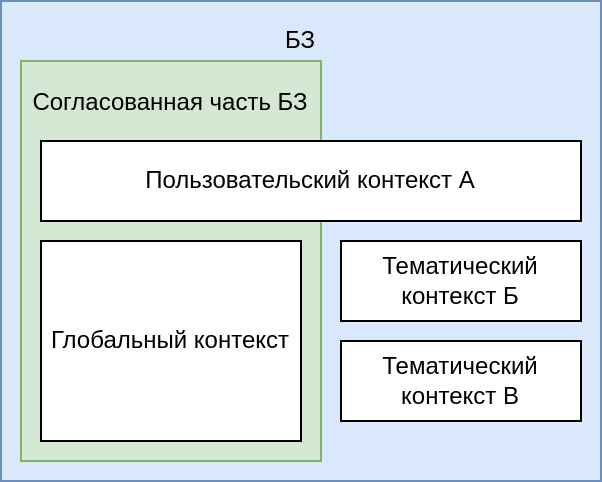
\includegraphics[width=0.4\textwidth]{images/part4/chapter_nl_interfaces/context_in_KB.png}
    \caption{Соотношение контекстов с согласованной частью баз знаний.}
    \label{fig:context_in_KB}
\end{figure}

\begin{SCn}

    \scnheader{контекст диалога}
    \scnrelfrom{subdividing}{\scnkeyword{Типология контекство по сроку достоверности знаний\scnsupergroupsign}}
    \begin{scnindent}
        \begin{scneqtoset}
            \scnitem{неизменяемый в ходе работы системы контекст диалога}
            \scnitem{изменяемый в ходе работы системы контекст диалога}
        \end{scneqtoset}
    \end{scnindent}

\end{SCn}

\textit{Неизменяемый в ходе работы системы контекст диалога} содержит в себе знания, необходимые для обеспечения выполнения системой своих функций,  которые были заложены в нее априорно ее разработчиками и/или администраторами и не изменяются в ходе ее функционирования на постоянной основе.

\textit{Изменяемый в ходе работы системы контекст диалога} содержит в себе знания, необходимые для обеспечения выполнения системой своих функций,  которые были ей получены в ходе ее работы и/или достоверность которых скоротечна.

\begin{SCn}


    \scnheader{изменяемый в ходе работы системы контекст диалога}
    \scnrelfrom{subdividing}{\scnkeyword{Типология изменяемых в ходе работы системы контекстов по источнику знаний\scnsupergroupsign}}
    \begin{scnindent}
        \begin{scneqtoset}
            \scnitem{контекст диалога, содержащий знания из внешних источников}
            \scnitem{контекст диалога, содержащий знания, полученные в ходе диалога}
        \end{scneqtoset}
    \end{scnindent}
    \scnrelfrom{subdividing}{\scnkeyword{Типология изменяемых контекстов по степени их достоверности\scnsupergroupsign}}
    \begin{scnindent}
        \begin{scneqtoset}
            \scnitem{достоверный контекст диалога}
            \scnitem{недостоверный контекст диалога}
        \end{scneqtoset}
    \end{scnindent}

\end{SCn}

Подмножество контекста может включаться в согласованную часть БЗ, например, если речь идет о каких-то предварительно занесенных в БЗ биографических сведениях -- дате рождения и т. п.

В каждый момент времени с пользователем связан 1 пользовательский диалоговый контекст (содержащий, по крайней мере известные заранее факты о нем: имя, возраст и т. п.) и несколько тематических.
Пример спецификации контекстов представлен на рисунке \textit{\nameref{fig:user_context}}.

\begin{figure}[h]
    \centering
    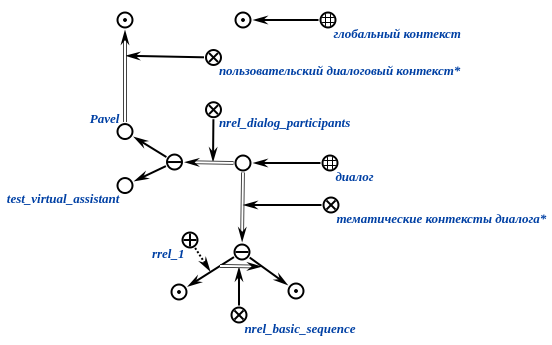
\includegraphics[width=0.5\textwidth]{images/part4/chapter_nl_interfaces/user_context.png}
    \caption{Пример спецификации контекстов.}
    \label{fig:user_context}
\end{figure}

Так, \textbf{действие. разрешение контекста} сводится к сопоставлению каждому варианту его значения соответствующего контекста.
Выбор производится на основании значения функции $F_{CTD}(T, C)$, где T - вариант трансляции, C - тематический контекст.
Подходящим контекстом для варианта трансляции считается тот, для которого значение этой функции максимально.
В случае, если подходящий контекст не найден, генерируется новый.
Пример результата данного действия представлен на рисунке \textit{\nameref{fig:relevant_contexts}}.

\begin{figure}[h]
    \centering
    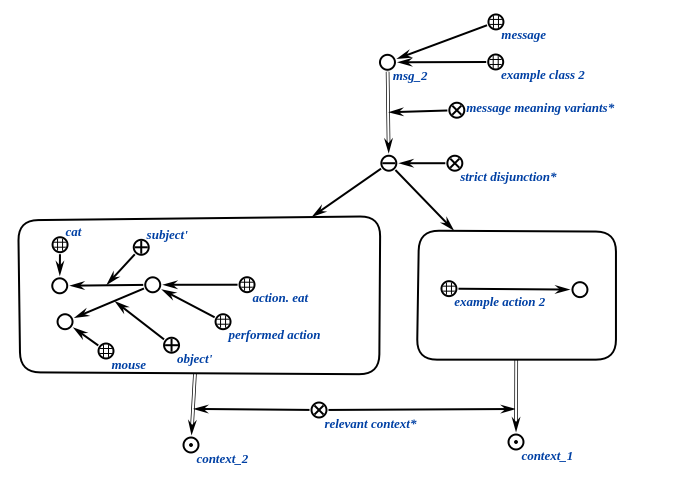
\includegraphics[width=0.45\textwidth]{images/part4/chapter_nl_interfaces/relevant_contexts.png}
    \caption{Пример сообщения, всем вариантам значения которого сопоставлен контекст.}
    \label{fig:relevant_contexts}
\end{figure}

\textbf{Действие. выбор смысла сообщения} представляет собой выбор из множества вариантов трансляции и соответствующих им контекстов одной пары и обозначение ее как эквивалентной сообщению конструкции. В простейшем случае, на данном этапе допустимо выполнить выбор в соответствии с рассчитанными на предыдущем этапе для пар потенциально эквивалентных структур и соответствующих им контекстов значениями функции $F_{CTD}(T, C)$ и выбрать пару, для которой оно максимально, однако при необходимости также возможно введение и отдельной функции.
Пример результата данного действия представлен на рисунке \textit{\nameref{fig:message_equivalent_structure}}.

\begin{figure}[h]
    \centering
    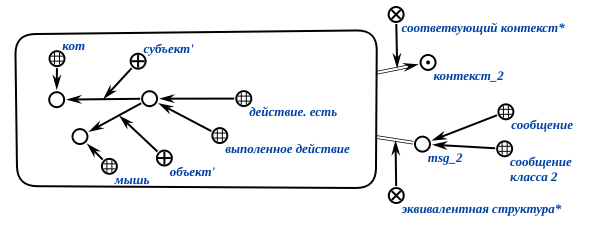
\includegraphics[width=0.35\textwidth]{images/part4/chapter_nl_interfaces/message_equivalent_structure.png}
    \caption{Пример конструкции, описывающей эквивалентную сообщению структуру.}
    \label{fig:message_equivalent_structure}
\end{figure}

\textbf{Действие. погружение сообщения в контекст} представляет собой погружение полученного смысла сообщения в контекст.
Кроме выбранного смысла сообщения, в контекст может добавляться и иная необходимая для обработки сообщения информация.
Кроме того, на данном этапе на основе хранящихся в контексте сведений также должно выполняться разрешение местоимений.
Примеры контекста до погружения в него сообщения и после погружения представлены на рисунках \textit{\nameref{fig:context_before_update}} и \textit{\nameref{fig:updated_context}}.

\begin{figure}[h]
    \centering
    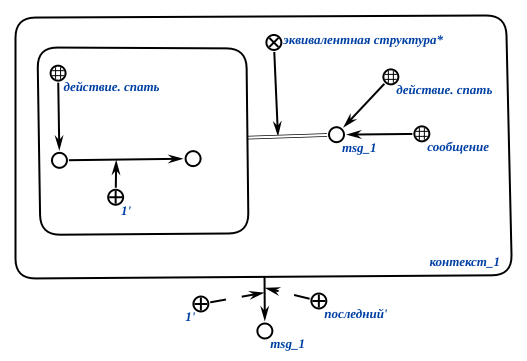
\includegraphics[width=0.4\textwidth]{images/part4/chapter_nl_interfaces/context_1.png}
    \caption{Пример контекста до погружения сообщения.}
    \label{fig:context_before_update}
\end{figure}

\begin{figure*}[h]
    \centering
    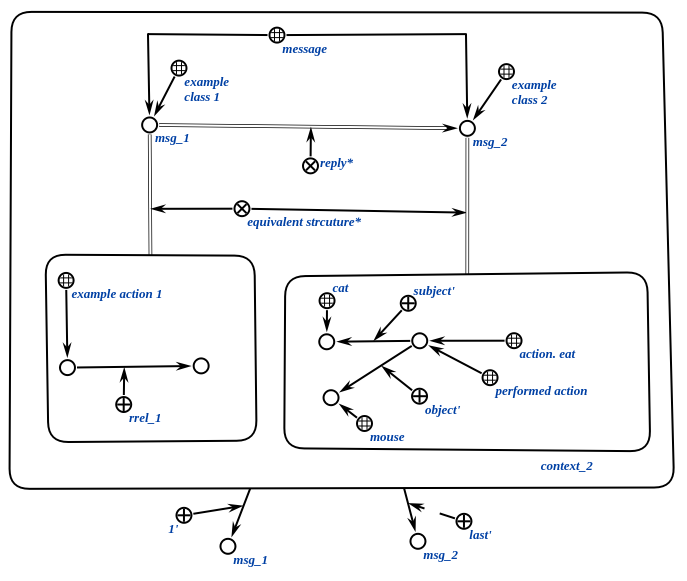
\includegraphics[width=0.7\textwidth]{images/part4/chapter_nl_interfaces/context_2.png}
    \caption{Пример контекста после погружения сообщения.}
    \label{fig:updated_context}
\end{figure*}

Таким образом, актуальная информация собирается в тематический контекст, объединив который с контекстом пользователя и глобальным контекстом можно получить общий контекст, на основании которого должны осуществляться требуемые действия системы, включая генерацию ответа системы.

%Под вопросом
\section{Предметная область и онтология синтеза естественно-языковых сообщений ostis-системы}
\section{Модели, методы и средства адаптации пользовательских интерфейсов к носителям китайского языка}
\label{section_chinese_interfaces}

%%%%%%%%%%%%%%%%%%%%%%%%% referenc.tex %%%%%%%%%%%%%%%%%%%%%%%%%%%%%%
% sample references
% %
% Use this file as a template for your own input.
%
%%%%%%%%%%%%%%%%%%%%%%%% Springer-Verlag %%%%%%%%%%%%%%%%%%%%%%%%%%
%
% BibTeX users please use
% \bibliographystyle{}
% \bibliography{}
%
\biblstarthook{In view of the parallel print and (chapter-wise) online publication of your book at \url{www.springerlink.com} it has been decided that -- as a genreral rule --  references should be sorted chapter-wise and placed at the end of the individual chapters. However, upon agreement with your contact at Springer you may list your references in a single seperate chapter at the end of your book. Deactivate the class option \texttt{sectrefs} and the \texttt{thebibliography} environment will be put out as a chapter of its own.\\\indent
References may be \textit{cited} in the text either by number (preferred) or by author/year.\footnote{Make sure that all references from the list are cited in the text. Those not cited should be moved to a separate \textit{Further Reading} section or chapter.} If the citatiion in the text is numbered, the reference list should be arranged in ascending order. If the citation in the text is author/year, the reference list should be \textit{sorted} alphabetically and if there are several works by the same author, the following order should be used:
\begin{enumerate}
\item all works by the author alone, ordered chronologically by year of publication
\item all works by the author with a coauthor, ordered alphabetically by coauthor
\item all works by the author with several coauthors, ordered chronologically by year of publication.
\end{enumerate}
The \textit{styling} of references\footnote{Always use the standard abbreviation of a journal's name according to the ISSN \textit{List of Title Word Abbreviations}, see \url{http://www.issn.org/en/node/344}} depends on the subject of your book:
\begin{itemize}
\item The \textit{two} recommended styles for references in books on \textit{mathematical, physical, statistical and computer sciences} are depicted in ~\cite{science-contrib, science-online, science-mono, science-journal, science-DOI} and ~\cite{phys-online, phys-mono, phys-journal, phys-DOI, phys-contrib}.
\item Examples of the most commonly used reference style in books on \textit{Psychology, Social Sciences} are~\cite{psysoc-mono, psysoc-online,psysoc-journal, psysoc-contrib, psysoc-DOI}.
\item Examples for references in books on \textit{Humanities, Linguistics, Philosophy} are~\cite{humlinphil-journal, humlinphil-contrib, humlinphil-mono, humlinphil-online, humlinphil-DOI}.
\item Examples of the basic Springer style used in publications on a wide range of subjects such as \textit{Computer Science, Economics, Engineering, Geosciences, Life Sciences, Medicine, Biomedicine} are ~\cite{basic-contrib, basic-online, basic-journal, basic-DOI, basic-mono}. 
\end{itemize}
}

\begin{thebibliography}{99.}%
% and use \bibitem to create references.
%
% Use the following syntax and markup for your references if 
% the subject of your book is from the field 
% "Mathematics, Physics, Statistics, Computer Science"
%
% Contribution 
\bibitem{science-contrib} Broy, M.: Software engineering --- from auxiliary to key technologies. In: Broy, M., Dener, E. (eds.) Software Pioneers, pp. 10-13. Springer, Heidelberg (2002)
%
% Online Document
\bibitem{science-online} Dod, J.: Effective substances. In: The Dictionary of Substances and Their Effects. Royal Society of Chemistry (1999) Available via DIALOG. \\
\url{http://www.rsc.org/dose/title of subordinate document. Cited 15 Jan 1999}
%
% Monograph
\bibitem{science-mono} Geddes, K.O., Czapor, S.R., Labahn, G.: Algorithms for Computer Algebra. Kluwer, Boston (1992) 
%
% Journal article
\bibitem{science-journal} Hamburger, C.: Quasimonotonicity, regularity and duality for nonlinear systems of partial differential equations. Ann. Mat. Pura. Appl. \textbf{169}, 321--354 (1995)
%
% Journal article by DOI
\bibitem{science-DOI} Slifka, M.K., Whitton, J.L.: Clinical implications of dysregulated cytokine production. J. Mol. Med. (2000) doi: 10.1007/s001090000086 
%
\bigskip

% Use the following (APS) syntax and markup for your references if 
% the subject of your book is from the field 
% "Mathematics, Physics, Statistics, Computer Science"
%
% Online Document
\bibitem{phys-online} J. Dod, in \textit{The Dictionary of Substances and Their Effects}, Royal Society of Chemistry. (Available via DIALOG, 1999), 
\url{http://www.rsc.org/dose/title of subordinate document. Cited 15 Jan 1999}
%
% Monograph
\bibitem{phys-mono} H. Ibach, H. L\"uth, \textit{Solid-State Physics}, 2nd edn. (Springer, New York, 1996), pp. 45-56 
%
% Journal article
\bibitem{phys-journal} S. Preuss, A. Demchuk Jr., M. Stuke, Appl. Phys. A \textbf{61}
%
% Journal article by DOI
\bibitem{phys-DOI} M.K. Slifka, J.L. Whitton, J. Mol. Med., doi: 10.1007/s001090000086
%
% Contribution 
\bibitem{phys-contrib} S.E. Smith, in \textit{Neuromuscular Junction}, ed. by E. Zaimis. Handbook of Experimental Pharmacology, vol 42 (Springer, Heidelberg, 1976), p. 593
%
\bigskip
%
% Use the following syntax and markup for your references if 
% the subject of your book is from the field 
% "Psychology, Social Sciences"
%
%
% Monograph
\bibitem{psysoc-mono} Calfee, R.~C., \& Valencia, R.~R. (1991). \textit{APA guide to preparing manuscripts for journal publication.} Washington, DC: American Psychological Association.
%
% Online Document
\bibitem{psysoc-online} Dod, J. (1999). Effective substances. In: The dictionary of substances and their effects. Royal Society of Chemistry. Available via DIALOG. \\
\url{http://www.rsc.org/dose/Effective substances.} Cited 15 Jan 1999.
%
% Journal article
\bibitem{psysoc-journal} Harris, M., Karper, E., Stacks, G., Hoffman, D., DeNiro, R., Cruz, P., et al. (2001). Writing labs and the Hollywood connection. \textit{J Film} Writing, 44(3), 213--245.
%
% Contribution 
\bibitem{psysoc-contrib} O'Neil, J.~M., \& Egan, J. (1992). Men's and women's gender role journeys: Metaphor for healing, transition, and transformation. In B.~R. Wainrig (Ed.), \textit{Gender issues across the life cycle} (pp. 107--123). New York: Springer.
%
% Journal article by DOI
\bibitem{psysoc-DOI}Kreger, M., Brindis, C.D., Manuel, D.M., Sassoubre, L. (2007). Lessons learned in systems change initiatives: benchmarks and indicators. \textit{American Journal of Community Psychology}, doi: 10.1007/s10464-007-9108-14.
%
%
% Use the following syntax and markup for your references if 
% the subject of your book is from the field 
% "Humanities, Linguistics, Philosophy"
%
\bigskip
%
% Journal article
\bibitem{humlinphil-journal} Alber John, Daniel C. O'Connell, and Sabine Kowal. 2002. Personal perspective in TV interviews. \textit{Pragmatics} 12:257--271
%
% Contribution 
\bibitem{humlinphil-contrib} Cameron, Deborah. 1997. Theoretical debates in feminist linguistics: Questions of sex and gender. In \textit{Gender and discourse}, ed. Ruth Wodak, 99--119. London: Sage Publications.
%
% Monograph
\bibitem{humlinphil-mono} Cameron, Deborah. 1985. \textit{Feminism and linguistic theory.} New York: St. Martin's Press.
%
% Online Document
\bibitem{humlinphil-online} Dod, Jake. 1999. Effective substances. In: The dictionary of substances and their effects. Royal Society of Chemistry. Available via DIALOG. \\
http://www.rsc.org/dose/title of subordinate document. Cited 15 Jan 1999
%
% Journal article by DOI
\bibitem{humlinphil-DOI} Suleiman, Camelia, Daniel C. O'Connell, and Sabine Kowal. 2002. `If you and I, if we, in this later day, lose that sacred fire...': Perspective in political interviews. \textit{Journal of Psycholinguistic Research}. doi: 10.1023/A:1015592129296.
%
%
%
\bigskip
%
%
% Use the following syntax and markup for your references if 
% the subject of your book is from the field 
% "Computer Science, Economics, Engineering, Geosciences, Life Sciences"
%
%
% Contribution 
\bibitem{basic-contrib} Brown B, Aaron M (2001) The politics of nature. In: Smith J (ed) The rise of modern genomics, 3rd edn. Wiley, New York 
%
% Online Document
\bibitem{basic-online} Dod J (1999) Effective Substances. In: The dictionary of substances and their effects. Royal Society of Chemistry. Available via DIALOG. \\
\url{http://www.rsc.org/dose/title of subordinate document. Cited 15 Jan 1999}
%
% Journal article by DOI
\bibitem{basic-DOI} Slifka MK, Whitton JL (2000) Clinical implications of dysregulated cytokine production. J Mol Med, doi: 10.1007/s001090000086
%
% Journal article
\bibitem{basic-journal} Smith J, Jones M Jr, Houghton L et al (1999) Future of health insurance. N Engl J Med 965:325--329
%
% Monograph
\bibitem{basic-mono} South J, Blass B (2001) The future of modern genomics. Blackwell, London 
%
\end{thebibliography}
